\subsection{Incenter Locus Recap}

Consider an EB centered at $O$, and an $N=3$ orbit, shown in Figure~\ref{fig:single-orbit}. A vertex bisector is congruent with the inward normal to the ellipse, and these meet at the orbit's Incenter $X_1$.

\begin{figure}[H]
     \centering
     \begin{subfigure}[t]{0.45\textwidth}
         \centering
         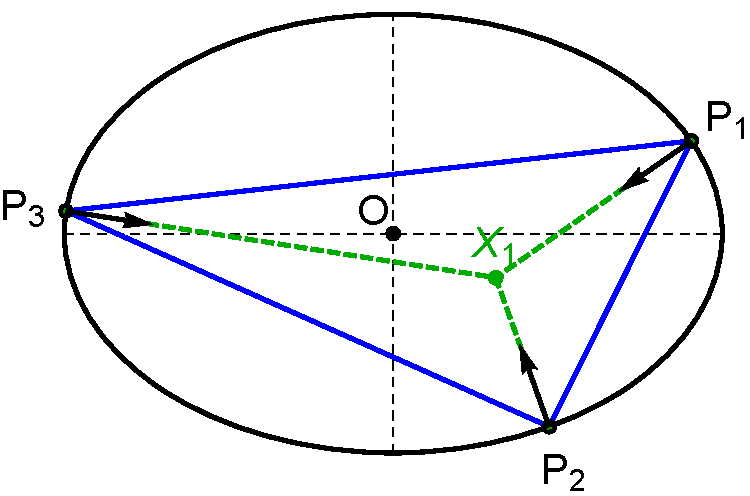
\includegraphics[height=.65 \linewidth]{pics/u0000_single_orbit.pdf}
         \caption{An $N=3$ {\em orbit}, and its Incenter $X_1$: where the bisectors concur.}
         \label{fig:single-orbit}
     \end{subfigure}
     \hfill
     \begin{subfigure}[t]{0.45\textwidth}
         \centering
          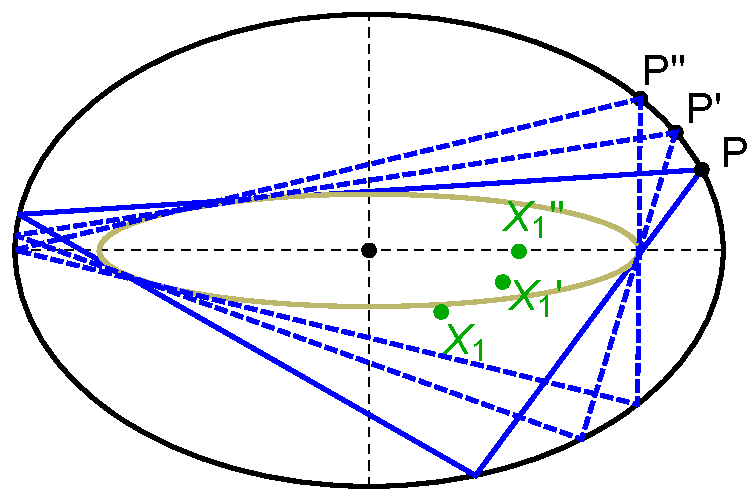
\includegraphics[height=.65\linewidth]{pics/u0010_three_orbits.pdf}
         \caption{Three triangular orbits, each identified by a starting vertex $P,P',P''$, and their Incenters $X_1,X_1',X_1''$, and the confocal Caustic.
         \label{fig:three-orbits}}
     \end{subfigure}
     \caption{Triangular Orbits in an EB and their Incenter. \href{https://youtu.be/Y3q35DObfZU}{Video} \cite[pl\#6]{dsr_math_intell_playlist}}
      \label{fig:6}
\end{figure}

Consider the three $N=3$ orbits in Figure~\ref{fig:three-orbits}, identified by a starting vertex $P,P',P''$, as well as their Incenters $X_1,X_1',X_1''$.

The Incenter's Cartesian coordinates in terms of a parametrized vertex, say $P(t)$, are a rather long, non-linear expression \cite{ronaldo19}. This renders remarkable the fact that its locus is an ellipse \cite{olga14} as are those of the Barycenter $X_2$, Circumcenter $X_3$, and Orthocenter $X_4$ \cite{corentin19,ronaldo19,sergei2016}. Recently, the following was also proven \cite{ronaldo19a}:

\begin{theorem}
The locus of the center $X_5$ of the 9-point circle is an ellipse.
\end{theorem}

The above can be seen in Figure~\ref{fig:locus-x12345} and in \cite[pl\#7]{dsr_math_intell_playlist}. Indeed, numerical analysis of the first 100 Kimberling Centers (only 39,900 to go) reported that only 29 of them produce elliptic loci \cite{ronaldo19a}.

\begin{figure}[H]
     \centering
     \begin{subfigure}[m]{0.45\textwidth}
     \centering
     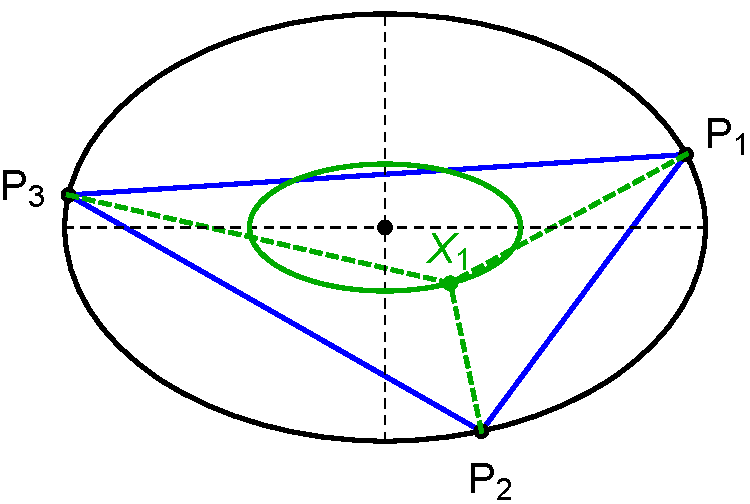
\includegraphics[height=.65\linewidth]{pics/u0020_incenter_locus.pdf}
         \caption{The locus of the Incenter $X_1$ is an ellipse. \href{https://www.youtube.com/watch?v=BBsyM7RnswA}{Video} \cite[pl\#2]{dsr_math_intell_playlist}}
        \label{fig:locus-incenter}
     \end{subfigure}
     \hfill
     \begin{subfigure}[m]{0.45\textwidth}
         \centering
         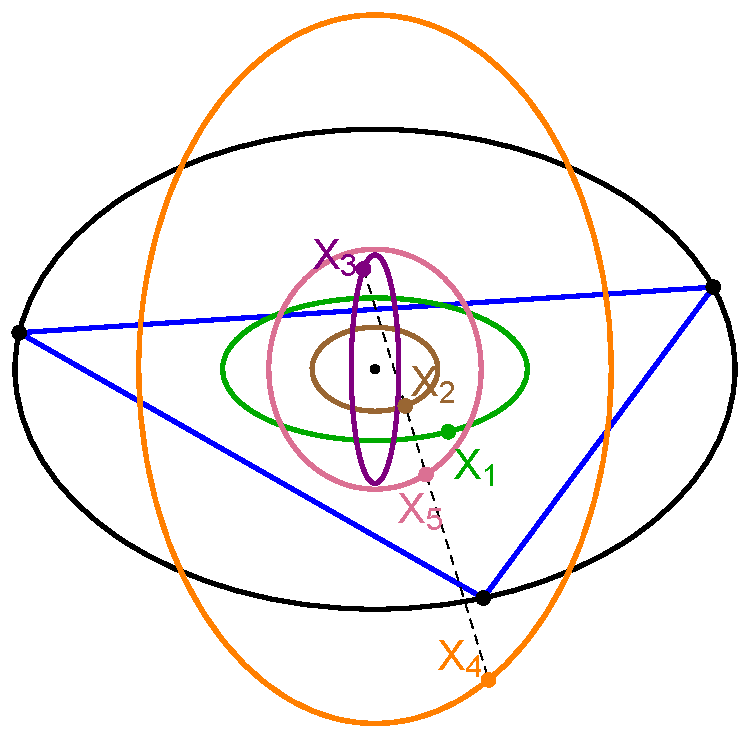
\includegraphics[height=\linewidth]{pics/u0030_x12345_locus.pdf}
         \caption{The loci of Incenter $X_1$, Barycenter $X_2$, Circumcenter $X_3$, Orthocenter $X_4$, and Center of the 9-Point Circle $X_5$ are all ellipses. \href{https://youtu.be/sMcNzcYaqtg}{Video} \cite[pl\#7]{dsr_math_intell_playlist}}
         \label{fig:locus-x12345}
     \end{subfigure}
     \caption{Loci of major triangle centers are ellipses.}
     \label{fig:7}
\end{figure}
%
\subsection{Eccentric Excenters}

The {\em Excenters} are defined in Figure~\ref{fig:constructions}. As depicted in Figure~\ref{fig:locus-incenter-excenter}, it can be shown that \cite{ronaldo19}:

\begin{theorem}
The locus of the Excenters is an ellipse similar to a rotated version of the Incenter's.
\end{theorem}
%
%
\begin{figure}[H]
    \centering
    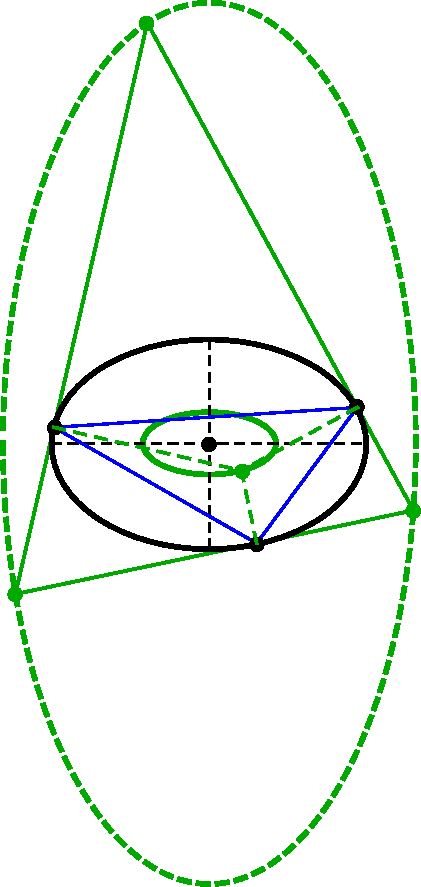
\includegraphics[angle=90,width=.66\textwidth]{pics/u0025_incenter_excenter_locus.pdf}
    \caption{An EB (black) is shown with its axes rotated (to save space), as well as an $N=3$ orbit (blue) and its Excentral Triangle (solid green). The locus of Excenters (vertices of the Excentral Triangle) is an ellipse similar to a perpendicular copy of the locus of the Incenter (shown solid green inside the EB). \href{https://youtu.be/Xxr1DUo19_w}{Video} \cite[pl\#8]{dsr_math_intell_playlist}}
    \label{fig:locus-incenter-excenter}
\end{figure}
%

The Excentral Triangle is an example of a {\em Derived Triangle}, i.e., its vertices are computed taking the orbit as a reference triangle. Generally, we've found that vertices of such triangles produce non-elliptic loci, with the Excentral Triangle being an exception. Consider the locus of the {\em Intouch Triangle}.
%\footnote{Points of contact of the Incircle with sides, known as {\em Intouchpoints}.}
As mentioned above, their locus is a self-intersecting sextic \cite[pl\#2]{dsr_math_intell_playlist}. In the same vein, vertices of the {\em Feuerbach Triangle}
%\footnote{Points of contact of the 9-Pt Circle with the Excircles, not to be confused with the Feuerbach {\em Point} $X_{11}$} 
and {\em Medial Triangle}
%\footnote{Triad of side midpoints} 
both produce non-elliptic loci, Figure~\ref{fig:non-elliptic}. Surprisingly \cite{ronaldo19a}:

\begin{theorem}
The locus of the vertices of the {\em Extouch Triangle}, where Excircles touch the orbit sides, is an ellipse identical to the Caustic.
\label{thm:extouch}
\end{theorem}

\begin{figure}[H]
    \centering
    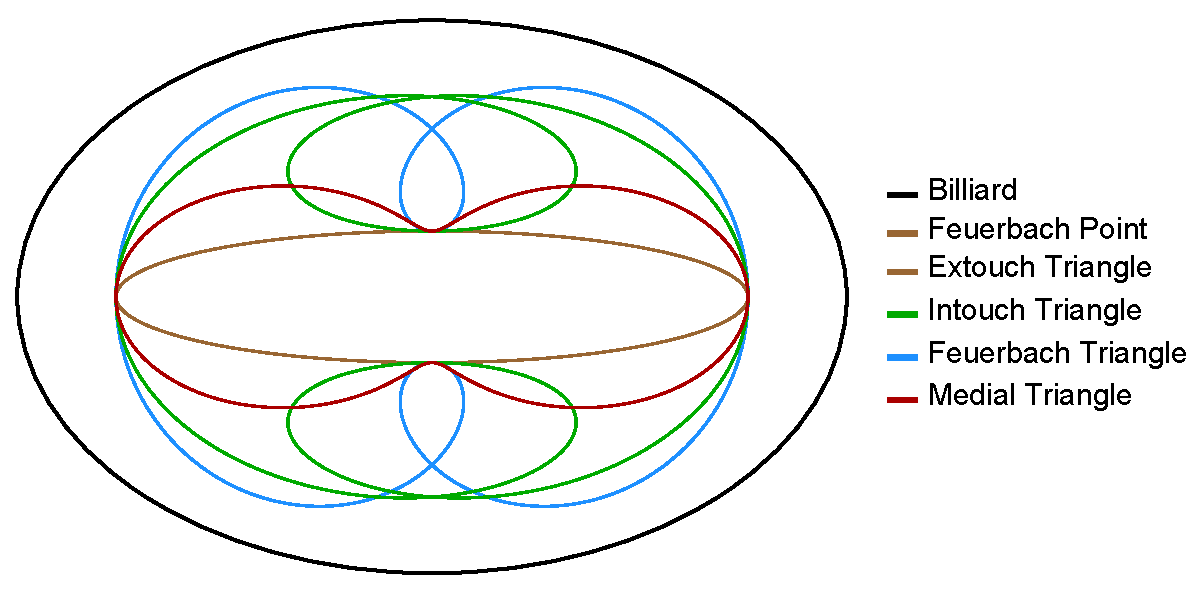
\includegraphics[height=.4\linewidth]{pics/u0040_non_elliptic.pdf}
    \caption{The vertices of the Intouch (green), Feuerbach (blue), and Medial (red) Triangles produce non-elliptic loci. Surprisingly, the Extouchpoints as well as the Feuerbach Point $X_{11}$ (both shown brown), are identical to the $N=3$ Caustic.
    %Note: the Feuerbach {\em Point} is where the 9-Point Circle touches the Incircle. 
    %The vertices of the Feuerbach {\em Triangle} are the contact points of the 9-Point Circle with the Excircles. 
    \href{https://youtu.be/OGvCQbYqJyI}{Video} \cite[pl\#9]{dsr_math_intell_playlist}}
    \label{fig:non-elliptic}
\end{figure}

\subsection{Fiery Feuerbach}

The Feuerbach Point $X_{11}$  is shown in Figure~\ref{fig:constructions}. $X_{100}$ is its {\em anticomplement}\footnote{A point's double-length reflection about the Barycenter $X_2$.}. As depicted in Figure~\ref{fig:feuer_loci}, 
this duo produces 
%produces 
a striking phenomenon \cite{ronaldo19a}:

\begin{theorem}
The locus of the Feuerbach Point $X_{11}$ is identical to the $N=3$ Caustic and the locus of its anticomplement $X_{100}$ is identical to the Billiard.
\end{theorem}

We also noticed that if orbit vertices slide along the Billiard in one direction, $X_{11}$ (resp. the Extouchpoints) will move along the Caustic in the opposite (resp. same) direction, depicted on this \href{https://youtu.be/TXdg7tUl8lc}{video} \cite[pl\#10]{dsr_math_intell_playlist}.

\begin{figure}[H]
    \centering
    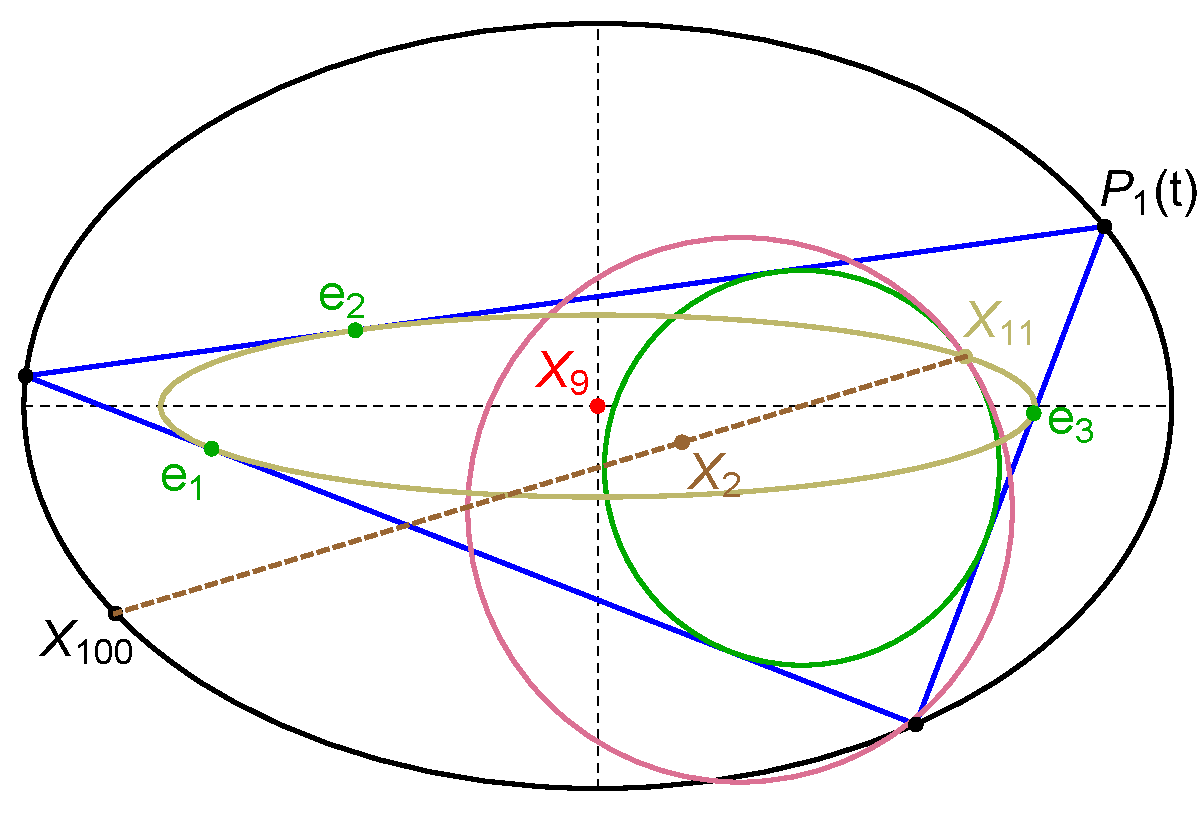
\includegraphics[width=.60\textwidth]{pics/u0035_feuerbach_loci.pdf}
    \caption{The EB (black), as well as an $N=3$ orbit (blue), with $P_1$ the starting vertex, and the Caustic (brown). Also shown are the orbit's Incircle (green) and 9-Point Circle (pink), whose single point of contact is the Feuerbach Point $X_{11}$. Shown also is its anticomplement $X_{100}$, and the three Extouchpoints $e_1,e_2,e_3$. Remarkable properties include: $X_{11}$ and the Extouchpoints sweep the Caustic, and $X_{100}$ sweeps the Billiard (in opposite directions).
    % done
    \href{https://youtu.be/TXdg7tUl8lc}{Video} \cite[pl\#12]{dsr_math_intell_playlist}}
    \label{fig:feuer_loci}
\end{figure}

\noindent Other interesting loci worthy of mention include:

\begin{itemize}
    \item Symmedian Point\footnote{Point of concurrence of a triangle's {\em symmedians}, i.e., the reflection of medians about the bisectors.} $X_6$: a convex quartic. When $1<a/b<2$ it closely approximates a perfect ellipse.
    \item Orthic's Incenter: a piecewise-elliptic locus with 4 kinks, shown in a  \href{https://youtu.be/3qJnwpFkUFQ}{video} \cite[pl\#11]{dsr_math_intell_playlist}
    \item Intouchpoints of the Anticomplementary Triangle: identical to the Billiard \cite{minevich17}, shown in a \href{https://youtu.be/50dyxWJhfN4}{video} \cite[pl\#12]{dsr_math_intell_playlist} 
\end{itemize}

\noindent The reader can easily observe the above with our \href{https://editor.p5js.org/undefined/present/i1Lin7lt7}{applet} \cite{dsr_applet_x12345}. 